\documentclass[pdflatex,sn-basic,Numbered]{sn-jnl}

\usepackage{graphicx}
\usepackage{amsmath}
\usepackage[table]{xcolor}
\usepackage{booktabs}
\usepackage{threeparttable}
\usepackage{tabularx}
\usepackage{array}
\usepackage{microtype}
\usepackage{placeins}
\usepackage{xurl}
\usepackage{multicol}

% Compact only front-matter gaps so the abstract and keywords share page one.
\usepackage{etoolbox}
\makeatletter
\patchcmd{\@maketitle}{\vskip20pt\artauthors}{\vskip12pt\artauthors}{}{\PackageError{jiis-layout}{Author spacing patch failed}{Check sn-jnl title macro.}}
\patchcmd{\@maketitle}{\vskip24pt}{\vskip16pt}{}{\PackageError{jiis-layout}{Email spacing patch failed}{Check sn-jnl title macro.}}
\patchcmd{\@maketitle}{\vskip24pt}{\vskip16pt}{}{\PackageError{jiis-layout}{Abstract spacing patch failed}{Check sn-jnl title macro.}}
\patchcmd{\abstracthead}{-22pt}{-16pt}{}{\PackageError{jiis-layout}{Abstract heading patch failed}{Check sn-jnl abstract macro.}}
\makeatother

\setlength{\textfloatsep}{10pt plus 2pt minus 2pt}
\setlength{\floatsep}{10pt plus 2pt minus 2pt}
\setlength{\intextsep}{10pt plus 2pt minus 2pt}

\hypersetup{
  bookmarksdepth=3,
  pdftitle={Reliability Boundaries of HyDE-Style Query Expansion in Multi-Hop Intelligent Information Retrieval},
  pdfauthor={Xingyun Chen; Shiyong Xiong},
  pdfkeywords={intelligent information retrieval; retrieval-augmented generation; multi-hop question answering; query expansion; reproducibility}
}

\newcommand{\best}[1]{\textbf{#1}}
% Generated; verified available evidence only.
\newcommand{\MHRBMAll}{0.583}
\newcommand{\MHRDenseAll}{0.503}
\newcommand{\MHRQAll}{0.448}
\newcommand{\MHRMAll}{0.434}
\newcommand{\MHRCEAll}{0.729}
\newcommand{\MHRCEGain}{0.146}

% Generated from the compiled supplement; rebuild after its numbering changes.
\newcommand{\SuppRef}[1]{\csname JIISsuppref@#1\endcsname}
\makeatletter
\@namedef{JIISsuppref@sec:ircot_fullwiki}{S4}
\@namedef{JIISsuppref@sec:supp_2wiki_paired_statistics}{S6}
\@namedef{JIISsuppref@sec:supp_answer_overlap_normalization}{S14}
\@namedef{JIISsuppref@sec:supp_code_artifact_availability}{S18}
\@namedef{JIISsuppref@sec:supp_deduplication_sensitivity}{S7}
\@namedef{JIISsuppref@sec:supp_dense_encoder_truncation}{S10.7}
\@namedef{JIISsuppref@sec:supp_detailed_sensitivity}{S12}
\@namedef{JIISsuppref@sec:supp_followup_holdout}{S27}
\@namedef{JIISsuppref@sec:supp_followup_serializer}{S26}
\@namedef{JIISsuppref@sec:supp_hotpotqa_paired_statistics}{S5}
\@namedef{JIISsuppref@sec:supp_independent_validation_new}{S25}
\@namedef{JIISsuppref@sec:supp_metric_normalization}{S13}
\@namedef{JIISsuppref@sec:supp_mhrag_external}{S20}
\@namedef{JIISsuppref@sec:supp_plan_b_sensitivity}{S3}
\@namedef{JIISsuppref@sec:supp_priority_diagnostics}{S23}
\@namedef{JIISsuppref@sec:supp_query_length_matched_hyde}{S15}
\@namedef{JIISsuppref@sec:supp_reader_controls_new}{S24}
\@namedef{JIISsuppref@sec:supp_sentence_audit}{S22}
\@namedef{JIISsuppref@sec:supp_verifier_guard_decomposition}{S8}
\@namedef{JIISsuppref@supp:sec:open_weight_confirmatory_protocol}{S2}
\@namedef{JIISsuppref@tab:claim_stress}{S54}
\@namedef{JIISsuppref@tab:evidence_completeness_buckets_supp}{S40}
\@namedef{JIISsuppref@tab:framework_comparison}{S55}
\@namedef{JIISsuppref@tab:priority_reader_controls}{S59}
\@namedef{JIISsuppref@tab:single_annotator_error_taxonomy}{S38}
\@namedef{JIISsuppref@tab:supporting_sentence_audit}{S56}
\makeatother


\begin{document}

\title[Reliability Boundaries of HyDE-Style Query Expansion]{Reliability Boundaries of HyDE-Style Query Expansion in Multi-Hop Intelligent Information Retrieval}

\author*[1]{\fnm{Shiyong} \sur{Xiong}}\email{1771856981@qq.com}
\author[1]{\fnm{Xingyun} \sur{Chen}}

\affil[1]{\orgdiv{School of Computer Science and Technology}, \orgname{Chongqing University of Posts and Telecommunications}, \orgaddress{\city{Chongqing}, \postcode{400065}, \country{China}}}

\abstract{Generative query expansion can improve retrieval without establishing corresponding gains in evidence delivered to readers or in multi-hop answer quality. We examine these configuration-specific reliability boundaries for Hypothetical Document Embeddings (HyDE)-style query expansion, using matched question-only baselines, complete-support retrieval, actual-input audits, and paired answer comparisons with family-specific Holm correction. In a frozen hosted HotpotQA artifact, HyDE raises all-support hit@10 from 0.630 to 0.868, but 292 of 500 generated passages contain exact answers; in separate matched BGE-encoder comparisons, two pinned 7B generators do not reproduce the hosted positive direction. In a random 300-question HotpotQA comparison excluding previously evaluated IDs and using a 5.23-million-paragraph corpus, cross-encoder reranking increases complete-support retrieval from 0.350 to 0.537 and exact-match accuracy by 9.0 percentage points with the Qwen reader and 7.0 with the Mistral reader, relative to BM25. HyDE improves retrieval, but its answer gain over BM25 remains unresolved with the Mistral reader. Cross-encoder retrieval gains on the 2WikiMultihopQA split-union corpus likewise do not establish answer gains. On MultiHop-RAG news documents, standard HyDE underperforms the matched question-only dense baseline in complete-support retrieval and all eight reader/length exact-match comparisons. In a separate matched 100-question HotpotQA intervention, a larger character budget increases complete-support retention from 46\% to 55\% without establishing answer gains. These findings distinguish retrieval, delivered evidence, and answers as separate validation targets within the tested configurations. The absence of an iterative-retrieval comparator on the external news corpus, incomplete cost measurements, and the absence of independent human validation constrain generalization.}
\keywords{intelligent information retrieval; retrieval-augmented generation; multi-hop question answering; query expansion; reproducibility}

\maketitle

\section{Introduction}
\label{sec:introduction}

Multi-hop intelligent information retrieval requires complete evidence acquisition. Retrieval-augmented generation (RAG)~\cite{lewis2020rag} grounds answers in external sources, but a multi-hop question can require documents linked by entities, comparisons or temporal relations. Missing one source may break the evidence chain despite a high rank for another. We therefore use complete supporting-title recovery as the primary retrieval diagnostic, supplemented by exact processed-record and evidence-interface audits.

Adaptive systems change queries or retrieve repeatedly to recover missing evidence. Multi-hop dense retrieval~\cite{xiong2021multihopdense} learns sequential evidence acquisition, and IRCoT~\cite{trivedi2022ircot} interleaves retrieval with reasoning. ReAct~\cite{yao2022react}, Self-RAG~\cite{asai2023selfrag} and Adaptive-RAG~\cite{jeong2024adaptiverag} add acting, reflection or complexity-based control, respectively. A final score alone cannot distinguish query representation, generator knowledge, corpus effects and additional calls. RCT-MARS~\cite{srivastava2026rctmars} shows that learned retrieval routing can fail to beat a strong fixed strategy, motivating matched diagnostics before crediting adaptive control.

HyDE~\cite{gao2022hyde} generates a hypothetical passage containing likely entities and relations for retrieval. Here the question and passage form the query; the reader receives only the original question and retrieved corpus evidence. This boundary keeps query generation separate from answer evidence. Case-based and concept-based retrieval~\cite{nasar2024retrieval} illustrates the role of representation and similarity choices, while BPLLM~\cite{bernardi2024bpllm} motivates component-wise validation in modular RAG systems. We study expansion as one such component.

The evaluation problem is conditional transport: which conclusions remain supported after a system component changes? Hosted aliases may drift, generated passages may reproduce benchmark content, and candidate pools may conceal corpus-scale difficulty. Data-centric AI~\cite{malerba2024datacentric} and FactualRAG~\cite{chang2026factualrag} motivate separating data and RAG-system evaluation concerns. The unresolved question here is whether matched expansion comparisons remain favorable when retrieved support passes through the actual reader interface. We examine this chain using complete-support retrieval, retained annotated evidence and paired answer scores. Generator, retriever, corpus, serializer, reader and budget identify each tested configuration. Existing paired inference supplies uncertainty; the contribution comes from the observed boundaries and their consequences for component evaluation.

We study four research questions. \textbf{RQ1:} Does HyDE-style expansion improve multi-hop evidence acquisition in the tested controlled pipelines? \textbf{RQ2:} How do matched gains differ across the tested generators? \textbf{RQ3:} Do retrieval conclusions survive full-wiki scale and an independently developed answer reader? \textbf{RQ4:} What evidence/answer trade-off appears as IRCoT receives more retrieval rounds? The corresponding contributions are:
\begin{enumerate}
\item \textbf{C1. Expansion against matched question-only baselines.} Controlled generator comparisons distinguish the hosted artifact from pinned open-generator estimates. News comparisons against the same question-only Dense retriever identify negative standard-expansion retrieval and answer effects. This tests expansion beyond comparison with a lexical baseline.
\item \textbf{C2. Retrieved versus delivered evidence.} Character and final-token audits locate losses that retrieval scores cannot reveal. A matched budget intervention increases annotated-support retention without establishing answer gains, separating delivery diagnostics from answer evaluation.
\item \textbf{C3. Retrieval versus answer gains.} Corpus-scale cross-encoder comparisons and two pinned readers identify configurations with supported retrieval gains but unresolved answer gains. Reader controls provide a separate capability reference, while round prefixes describe iteration under unequal accumulated cost.
\end{enumerate}

Here, reliability boundaries denote the empirical limits of supported retrieval and answer gains within the tested configurations. An unresolved gain is not evidence of no effect. Named contrasts, family-specific paired decisions and hashed records support inspection; they do not yield a universal account of when expansion works, a predictive model or a validated method-selection rule.

The tested English configurations comprise a complete HotpotQA Wikipedia snapshot, a 2Wiki official split-union corpus and MultiHop-RAG~\cite{tang2024multihoprag} news documents. The latter's local IRCoT condition is unavailable, and no independent human evidence-sufficiency validation was performed. Available conditions do not complete the registered transport test. The remainder of the article presents related work (Section~\ref{sec:related_work}), the protocol (Section~\ref{sec:method}), RQ1--RQ4 and external validation (Section~\ref{sec:experiments}), and interpretation and limits (Sections~\ref{sec:discussion_limitations}--\ref{sec:conclusion}).

\section{Related Work}
\label{sec:related_work}

\subsection{Intelligent Query Formulation and Retrieval}
\label{sec:rw_query_retrieval}

Dense Passage Retrieval~\cite{karpukhin2020dpr} and ColBERT~\cite{khattab2020colbert} learn representations for semantic matching; RAG~\cite{lewis2020rag} couples retrieved evidence with a reader. Case-based and concept-based retrieval~\cite{nasar2024retrieval} also depends on how cases, concepts and similarity functions are represented. We fix the retriever and index within each query-formulation comparison.

Generation-augmented retrieval~\cite{mao2020gar} expands questions with generated text; Query2doc~\cite{wang2023query2doc} generates pseudo-documents from demonstrations; Rewrite-Retrieve-Read~\cite{ma2023rewrite} rewrites queries; and HyDE~\cite{gao2022hyde} retrieves using hypothetical-document embeddings. Our question-only, rewrite, document-like, evidence-only and Query2doc-style conditions share frozen retrieval settings. The four-shot Query2doc-style condition is an adaptation, not an official reproduction or a new expansion algorithm.

\subsection{Multi-Hop and Iterative RAG Systems}
\label{sec:rw_multihop_iterative}

Multi-hop benchmarks make evidence completeness observable because answers depend on linked sources. HotpotQA~\cite{yang2018hotpotqa} supplies supporting facts, 2WikiMultihopQA~\cite{ho2020twowiki} exposes explicit reasoning chains, and MuSiQue~\cite{trivedi2021musique} composes questions from connected single-hop relations. Multi-hop dense retrieval~\cite{xiong2021multihopdense} learns sequential evidence acquisition; IRCoT~\cite{trivedi2022ircot} alternates reasoning and retrieval. ReAct~\cite{yao2022react}, FLARE~\cite{jiang2023flare}, Self-RAG~\cite{asai2023selfrag} and Adaptive-RAG~\cite{jeong2024adaptiverag} add action, confidence, reflection or complexity-based control, respectively. These approaches change both evidence acquisition and operating cost, so iteration must be distinguished from query representation.

BPLLM~\cite{bernardi2024bpllm} evaluates retrieval, chunking, prompts, embeddings and open-model choices within a modular information system. Following this component-wise view, our controlled tier isolates query representation; the full-wiki tier compares OneR/BM25, HyDE-BM25 and the official IRCoT state machine on one index. IRCoT retains official orchestration but replaces the historical generator with a pinned local model. Its round-prefix results are unequal-cost sensitivity, not an equal-budget stopping-policy trial.

\subsection{Reliability, Leakage, and Reproducibility of Generative Retrieval}
\label{sec:rw_reliability}

FRAMES~\cite{krishna-etal-2025-fact} evaluates factual retrieval, SetR~\cite{lee-etal-2025-shifting} studies evidence-set selection, and \emph{Stronger Baselines}~\cite{laitenberger-etal-2025-stronger} examines implementation-sensitive comparisons. RAGAS~\cite{es2023ragas} scores faithfulness, answer relevance and context relevance using automated judges. ARES~\cite{saadfalcon2023ares} trains component judges and uses human-labeled calibration with prediction-powered inference to estimate system quality. RAGChecker~\cite{ru2024ragchecker} decomposes responses and reference answers into claims, evaluating their entailment against responses and retrieved chunks. These approaches address semantic quality and component diagnostics; they already extend evaluation beyond a single answer score.

Our short-answer study measures a different object: same-question changes between specified configurations, including annotated support remaining in effective reader tokens. Exact retention complements semantic diagnostics but cannot replace entailment assessment or human evidence-sufficiency judgments. We neither run nor establish superior accuracy over these evaluation tools. RCT-MARS~\cite{srivastava2026rctmars} studies retrieval routing and soft fusion under quality--cost trade-offs. Our audit tests expansion references, delivered evidence and answer effects without learning a router. Its new-sample rules can select the same method, yielding no decision increment.

Yoon et al.~\cite{yoon2025knowledgeleakage} connect hypothetical-document gains to gold-evidence entailment in fact verification, using both retrieval and verdict-prediction outcomes. We build on this concern with multi-hop complete-support acquisition, character/token delivery and short-answer comparisons under matched retrievers. Our lexical content strata are narrower measurements than their entailment matching and cannot certify absence of paraphrased knowledge. FactualRAG~\cite{chang2026factualrag} documents retrieval-coverage limits and cross-model variation, and data-centric AI~\cite{malerba2024datacentric} emphasizes robustness, drift and reuse. Hosted-alias replay additionally limits our evidence to preserved outputs without identifying a causal contamination mechanism.

\section{Method}
\label{sec:method}

\subsection{Information-System Architecture and Evidence Boundary}
\label{sec:method_overview}

The system has four layers: query representation, corpus/index retrieval, evidence serialization and audit/evaluation (Figure~\ref{fig:method_pipeline}). Query representation produces a question vector, rewrite, hypothetical passage or iterative query. A frozen dense or BM25 index retrieves records; the serializer passes corpus evidence to a short-answer reader. Evaluation measures completeness, EM/F1, paired uncertainty, calls, content overlap and provenance. Query-composition diagnostics appear in Online Resource 1, Section~\SuppRef{sec:supp_answer_overlap_normalization}.

\begin{figure}[tbp]
\centering
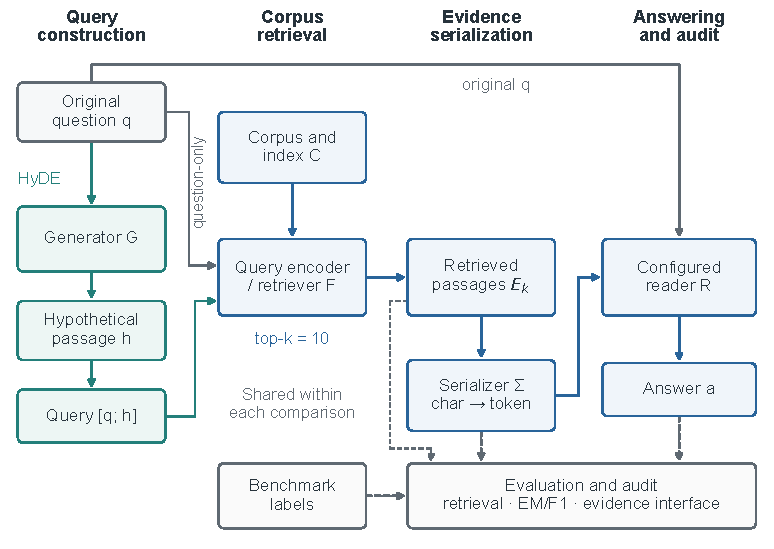
\includegraphics[width=\textwidth]{Fig1_Workflow.pdf}
\caption{System workflow and evidence boundary. Question-only and HyDE are separate conditions sharing the corpus, index, retrieval configuration and top-$k=10$ within each comparison. HyDE forms $[q;h]$ from the question $q$ and hypothetical passage $h$. The reader receives the original question and serialized corpus evidence under condition-specific character and token budgets. Solid arrows show inference; dashed arrows show evaluation and audit. Benchmark labels enter evaluation only. Optional answer postprocessing is omitted.}
\label{fig:method_pipeline}
\end{figure}


The controlled tier uses released candidate pools and a question-independent 100k pool; the HotpotQA full-wiki tier adds iterative retrieval on a 5.23-million-paragraph index. In the primary retrieval tiers, readers see only the original question and retrieved corpus evidence, excluding hypothetical documents, rewritten queries, gold markers and reasoning traces. Supporting-title completeness is primary; exact-record and serialized-evidence coverage are distinct diagnostics. The exploratory guarded answer-format analysis remains secondary (Online Resource 1, Section~\SuppRef{sec:supp_verifier_guard_decomposition}).

The audit identifies each system as $S=(G,F,C,\Sigma,R,B)$: generator, retrieval function, corpus/index, evidence serializer, reader and operating budget. An observed configuration edge carries source/target effects, metric direction, paired intervals, frozen sample identifiers and artifact hashes. Binary local decisions use two-sided exact paired tests with Holm adjustment within the declared family. Favorable significant effects support a local gain; adverse significant effects support its opposite direction. Other local decisions remain unresolved. Reader interactions use separately declared paired sign-flip tests where applicable; intervals estimate uncertainty rather than decide significance.

Transport additionally requires an eligible, favorable source effect with $p_{\mathrm{Holm}}<0.05$. Supported transport requires favorable adjusted decisions for all required target effects; contrary adjusted evidence can reject it, while absent or ineligible evidence leaves it unresolved. Thus a supported local reranker gain need not establish transport from the source configuration. Metrics remain separate, and changing multiple components prevents causal attribution. Table~\ref{tab:boundary_stability_matrix} names local contrasts underlying the overview; the complete CSV retains source-and-target classifications and hashes. This is an empirical audit workflow, not a new retrieval algorithm or statistical test.

\subsection{Formal Protocol and Boundaries}
\label{sec:formal_protocol}

For question $q$ and title--paragraph corpus $\mathcal{C}$, the generator produces $h=G(q)$. The primary dense query is $[q;h]$, ranked by $\mathrm{sim}(f([q;h]),f(d))$ to obtain top-$k$ corpus evidence $E_k$ and answer $a_0=R(q,E_k)$. Question-only, rewrite and hypothetical-only variants are diagnostics. The generated passage is a retrieval representation, not reader evidence; factual correctness and completeness are not guaranteed.

\subsection{Open-Weight Confirmatory Tier}
\label{sec:open_weight_confirmatory_tier}

The two local generators are revision-pinned Qwen2.5-7B-Instruct and Mistral-7B-Instruct-v0.3; revisions and prompts are recorded in Online Resource 1, Section~\SuppRef{supp:sec:open_weight_confirmatory_protocol}. Both use greedy decoding, seed 13 and a 96-token cap. The Qwen tier compares question-only Dense, standard HyDE, evidence-only HyDE and Query2doc-style (4-shot adaptation); deterministic target-dependent demonstration selection is documented in the supplement. Mistral repeats standard HyDE with the same question order, serialization and retrieval settings, without model-specific tuning.

All conditions hold BGE-base at revision \path{a5beb1e3e68b9ab74eb54cfd186867f64f240e1a}, CLS pooling, L2 normalization, a 512-token input limit and top-$k=10$ fixed. Evaluation gold answers and support flags are never supplied to the generator outside the explicitly fixed training demonstrations. This tier measures retrieval only; no reader result is inferred. Sanitized public rows retain stable IDs, condition, rank, document IDs, scores and metric fields while excluding benchmark text and unrestricted generations.

\subsection{Post-Hoc and Pre-Output Sensitivity Analyses}
\label{sec:review_driven_sensitivity}

Four additional sensitivity analyses were specified before inspecting their own outputs, after the initial study; they are not preregistered evidence. Retrospective evidence diagnostics are identified separately. Sample order is fixed; resampling uses seed 13 and 10,000 question-level draws, without result-dependent tuning or deletion.

The BGE instruction check changes only the recommended query prefix, with four all-support contrasts in one Holm family. Evidence-interface diagnostics separately measure complete-paragraph and retrospectively acquired official-sentence retention at 450/900 characters (Online Resource 1, Section~\SuppRef{sec:supp_sentence_audit}); neither establishes factual sufficiency.

Reader interactions use paired difference-in-differences, bootstrap intervals and separately specified sign-flip/Holm tests. The pinned \texttt{BAAI/bge-reranker-v2-m3} cross-encodes frozen 500-by-100 BM25 pools and returns ten records without generation. BGE-base rescoring is a separate bi-encoder control. Revisions, exact/Monte Carlo test variants and families are in Online Resource 1, Section~\SuppRef{sec:supp_plan_b_sensitivity}.

\subsection{Official-Code Full-Wiki Tier and Common Full-Wiki Reader}
\label{sec:fullwiki_common_reader}

HotpotQA full-wiki uses official IRCoT inference code at commit \path{3c1820f698eea5eeddb4fba3c56b64c961e063e4}, the pinned local Qwen generator, and a 5,233,329-paragraph Elasticsearch BM25 index. OneR/BM25, one-generation HyDE-BM25 and adaptive IRCoT share the index/evaluator. IRCoT retrieves two documents per round with the official exit controller and at most ten reasoning sentences; this is an official-code/open-generator adaptation, not historical replay.

A separate 500-question 2Wiki tier uses a question-independent index of 428,395 unique paragraphs from official train/dev/test contexts (English analyzer; BM25 $k_1=1.2$, $b=0.75$). It tests BM25, Qwen-HyDE, the same IRCoT adaptation and the learned cross-encoder on BM25 top-100. Adaptive stopping can return fewer than ten documents. This split-union corpus is not a second complete Wikipedia snapshot.

Both pinned readers consume frozen ranked evidence without rerunning retrieval or selecting examples. Qwen and Mistral use greedy seed 13, 2,000 input tokens and at most 32 new tokens; model revisions are listed in Online Resource 1. The shared prompt contains the question and at most ten title/paragraph blocks, each with a 450-character paragraph prefix. Gold answers, flags, hypothetical passages and reasoning traces are excluded. The local common-reader scorer maximizes EM/F1 over released aliases. A fixed deterministic adapter normalizes specified abstention markers, answer prefixes, quotation pairs and narrow trailing explanations; private raw predictions are preserved. Hosted processed-corpus rows instead use one gold string. The local scorer differs from official HotpotQA/2Wiki conventions; the pipeline map and retrospective comparison appear in Online Resource 1, Section~\SuppRef{sec:supp_metric_normalization}.

Within-reader HyDE/IRCoT-versus-OneR and cross-reader comparisons have separately declared Holm families, with 10,000 paired bootstrap resamples (seed 13) and exact McNemar tests for EM. Interactions are separately tested rather than inferred from rankings. Cost separates retrieval, query/chain generation and reader calls. The round-prefix sensitivity rescores frozen trajectories after rounds one and two and at natural/capped exit, using the same Qwen reader, paired intervals and separately adjusted binary retrieval/EM tests. Prefixes accumulate different calls and document counts; this is not an equal-budget experiment. Full adapters, deviations, stopping and privacy records appear in Online Resource 1, Section~\SuppRef{sec:ircot_fullwiki}.

\subsection{HyDE-Style Dense Retrieval}
\label{sec:hyde_retrieval}

The processed-corpus primary index encodes title plus paragraph with normalized Sentence-BERT~\cite{reimers2019sentencebert} embeddings from \texttt{all-MiniLM-L6-v2}, based on MiniLM~\cite{wang2020minilm}. FAISS~\cite{johnson2019billion} performs inner-product search, equivalent to cosine similarity for these normalized vectors. Question plus hypothetical passage (capped at 900 characters) shares the encoder's 256-token right-truncation policy across query variants (Online Resource 1, Section~\SuppRef{sec:supp_dense_encoder_truncation}). BGE is a separately labeled retriever and does not replace the frozen MiniLM artifacts.

\subsection{Evidence-Grounded Short-Answer LLM Reader}
\label{sec:short_answer_reader}

The reader sees the original question and ranked, character-budgeted corpus evidence, with instructions to combine facts and return a short answer using only those records. Fixed generic formatting instructions cover yes/no, location, date/age and role questions; they are shared across the processed HotpotQA and 2Wiki evaluations and contain no evaluation labels. Answers need not be contiguous spans. The hosted processed-corpus reader uses temperature-0 relay decoding; the separately pinned local readers and their token limits are specified in Section~\ref{sec:fullwiki_common_reader}.

\subsection{Implementation Details}
\label{sec:implementation_boundary}

All generation modules use fixed prompt templates. The HyDE prompt asks for one concise hypothetical supporting passage, and the reader prompt asks for an exact short answer from retrieved evidence only. For the processed-corpus study, the wrapper calls a third-party OpenAI-compatible relay exposing the API alias \texttt{qwen3.7-max} with \texttt{temperature=0.0}; local artifacts preserve that alias but provide no independently verified provider-side immutable snapshot. The reported \texttt{max\_tokens} settings are 64 for HyDE passage generation, 64 for rewritten-query generation, and 64 for reader answers. The prompt JSONL artifacts retain gold-answer metadata for evaluation and auditing, but the gold answer is not inserted into the prompt text shown to the model. We distinguish artifact-level reproducibility for hosted runs, executable local reproducibility for Qwen2.5-7B, and official-code/open-generator adaptation for IRCoT.

\textbf{AI assistance.} OpenAI Codex assisted experiment-code development and debugging, statistical/table reconstruction, manuscript drafting and revision, and local submission preparation. Its outputs are not independent human annotations or experimental measurements. Model-generated study answers are evaluated only under the disclosed experimental protocols. All AI-assisted outputs were reviewed and verified by the authors, who take full responsibility for the final code, analyses, results and manuscript.


\subsection{Versioned External Evidence and Incomplete Families}
\label{sec:mhrag_method_gate}

MultiHop-RAG uses parent evidence IDs, non-null retrieval/EM/F1 denominators and a separate null-abstention endpoint. The versioned correction budgets evidence while preserving the complete answer/chat suffix under frozen token limits; malformed historical outputs are excluded and verified token-identical reuse is explicit. Four observed contrasts retain an unavailable fifth IRCoT slot at 1.0 during Holm correction. A within-configuration effect is not a complete transport decision. Alternative prompts/seeds never replace primary conditions. The planned independent human audit was withdrawn after automated results were available because qualified annotators could not be recruited. No independent human validation was performed; benchmark labels and automated metrics do not establish human evidence sufficiency or annotation agreement. Full correction, parameter and cost records accompany the external-validation tables in Online Resource 1.

\subsection{New Diagnostic Reader Controls}
\label{sec:new_reader_controls_method}
After observing the historical results, we froze the first 100 IDs in the original HotpotQA order for question-only and gold-selected-support controls. Both pinned readers retain greedy seed 13 and a 32-token output cap. Gold prompts contain all official supporting sentences and titles, without the answer field, character clipping or input truncation. The maximum actual gold inputs are 298/314 tokens for Qwen/Mistral, within the original 2,000-token budget. These are capability references with different evidence selection and instructions, not strict upper bounds or causal retrieval ablations. New local/official EM/F1 families and raw/adapted outputs are reported separately in Online Resource 1, Section~\SuppRef{sec:supp_reader_controls_new}.

\subsection{Prospective Follow-up Comparisons}
\label{sec:followup_comparisons_method}
Separate protocols fix a same-question 100-example character-budget intervention (EM and F1 families of two each) and a random 300-example full-wiki method matrix. The latter excludes all 564 previously observed IDs and compares BM25, standard Qwen-HyDE/BM25 and the cross-encoder under both pinned readers. For this matrix, EM/F1 use the single official answer, rather than the broader released aliases of the historical tier. Primary EM, retrieval and secondary F1 use separate families of six, three and six tests; official sensitivities remain separate. Samples, power assumptions, failure rules and amendments frozen before model outputs are detailed in Online Resource 1, Sections~\SuppRef{sec:supp_followup_serializer} and~\SuppRef{sec:supp_followup_holdout}. New results remain separate from historical means.

\begin{table*}[t]
\centering
\caption{Named local contrasts underlying the reliability-boundary overview. Effects are target minus baseline, with paired 95\% intervals. Local decisions use the stated Holm family and do not themselves establish transport across configurations.}
\label{tab:boundary_stability_matrix}
\footnotesize
\begin{threeparttable}
\setlength{\tabcolsep}{3pt}
\renewcommand{\arraystretch}{1.10}
\begin{tabularx}{\textwidth}{>{\raggedright\arraybackslash}p{0.12\textwidth}>{\raggedright\arraybackslash}p{0.28\textwidth}>{\raggedright\arraybackslash}p{0.20\textwidth}>{\raggedright\arraybackslash}p{0.13\textwidth}>{\raggedright\arraybackslash}X}
\toprule
Factor / endpoint & Dataset and target versus baseline & $\Delta$ [95\% CI] & $p_{\mathrm{Holm}}$ & Local decision / scope \\
\midrule
Generator / AS & HotpotQA processed BGE: Qwen-HyDE vs Dense & $-0.036$ [$-0.062,-0.010$] & 0.0658 & unresolved; six-contrast generator family \\
Generator / AS & HotpotQA processed BGE: Mistral-HyDE vs Dense & $-0.034$ [$-0.064,-0.006$] & 0.1201 & unresolved; same family \\
Reranker / AS & HotpotQA full-wiki: cross-encoder vs HyDE & $+0.120$ [0.076, 0.162] & $3.26\!\times\!10^{-7}$ & supported local gain; BM25 top-100 pool \\
Reranker / AS & HotpotQA full-wiki: cross-encoder vs IRCoT & $+0.114$ [0.064, 0.164] & $2.77\!\times\!10^{-5}$ & supported local gain; same pool \\
Reranker / AS & HotpotQA full-wiki: cross-encoder vs BGE rescore & $+0.008$ [$-0.002$, 0.020] & 0.2891 & unresolved; bi-encoder comparator \\
Corpus / AS & 2Wiki split-union: cross-encoder vs BM25 & $+0.054$ [0.032, 0.078] & $2.23\!\times\!10^{-5}$ & supported retrieval gain; answer decisions unresolved \\
Reader / EM & HotpotQA full-wiki, Qwen: cross-encoder vs BM25 & $+0.044$ [0.014, 0.074] & 0.0214 & supported local answer gain \\
Reader / EM & HotpotQA full-wiki, Mistral: cross-encoder vs BM25 & $+0.060$ [0.032, 0.090] & 0.0003 & supported local answer gain; interaction unresolved \\
Budget / AS & HotpotQA IRCoT: full budget vs round two & $+0.010$ [0.002, 0.020] & 0.0625 & unresolved; unequal cumulative calls \\
\bottomrule
\end{tabularx}
\begin{tablenotes}
\footnotesize
\item All rows have $n=500$. AS means complete supporting-title recovery; EM means local answer exact match. Adjustments are family-specific. The first two rows use the six-contrast generator family; reranker retrieval, 2Wiki retrieval and each reader use their separate declared families.
\item The historical matrix assigns unresolved transport to the reranker factor despite supported individual gains. Full-paragraph losses at 450 characters are 0.246 (HyDE), 0.214 (IRCoT), and 0.284 (BGE rescore). They are non-primary diagnostics, not formal transport decisions; sentence and final-token audits appear separately in Online Resource 1.
\end{tablenotes}
\end{threeparttable}
\end{table*}

\section{Experiments}
\label{sec:experiments}

\subsection{Evaluation Protocol}
\label{sec:dataset_setting}

We evaluate four research questions using two 500-example processed Wikipedia benchmarks, full-wiki HotpotQA, the official 2Wiki split-union corpus and external news validation. Processed pools are jointly indexed but remain question-derived; the corpus-scale indexes are question-independent. The primary processed tier uses MiniLM, while generator comparisons fix BGE-base. Methods, reader interfaces and index sizes are specified in Section~\ref{sec:method}.

Retrieval outcomes are any supporting-title hit@10, all supporting-title hit@10, and mean supporting-title recall@10. We emphasize all-support hit and recall because multi-hop answering can fail when one required page is absent. Reader outcomes are normalized Exact Match (EM) and token F1. The hypothetical passage is used only to form a retrieval query and is never supplied to the reader as evidence. Exact normalized title--paragraph matching, corpus construction, deduplication, top-$k$, and leakage diagnostics are detailed in Online Resource 1, Sections~\SuppRef{sec:supp_deduplication_sensitivity}, \SuppRef{sec:supp_dense_encoder_truncation}, \SuppRef{sec:supp_metric_normalization} and~\SuppRef{sec:supp_answer_overlap_normalization}.

All confirmatory contrasts use paired examples. Effect intervals are question-level percentile bootstrap intervals with 10,000 resamples; binary paired outcomes use exact McNemar tests. Holm correction applies within each stated family. Allowlisted metric exports contain identifiers or their hashes, conditions, scores and provenance, excluding benchmark text and private predictions. Reconstruction coverage and missing inputs are listed separately in Online Resource 1, Section~\SuppRef{sec:supp_code_artifact_availability}.

Hosted results support frozen-artifact audit without an independently verified immutable provider snapshot. The local tiers use pinned weights; IRCoT and four-shot Query2doc-style are disclosed adaptations rather than historical reproductions. Their implementation boundaries are specified in Section~\ref{sec:implementation_boundary} and Online Resource 1.

The transportability axes remain bounded. HotpotQA uses a complete 2017 English Wikipedia index, whereas the 2Wiki corpus is frozen from released benchmark contexts and is not a second complete Wikipedia snapshot. The latter removes question-specific candidate pools and supplies an independent corpus-scale, cross-dataset test, but it does not establish transport to another complete Wikipedia collection or to a non-Wikipedia corpus.

\subsection{RQ1: Controlled Evidence Acquisition}
\label{sec:rq1_controlled_evidence}

The primary predeclared comparison asks whether one document-like expansion improves complete evidence acquisition relative to question-only Dense RAG under the frozen hosted-generator pipeline. On HotpotQA, HyDE raises all-support hit@10 from 0.6300 to 0.8680, a paired difference of $+0.2380$ (95\% CI $[0.2000,0.2780]$), and raises supporting-title recall from 0.8080 to 0.9280 ($+0.1200$; $[0.1010,0.1410]$). Reader EM/F1 increase from 0.5940/0.7199 to 0.6840/0.8105 (Online Resource 1, Section~\SuppRef{sec:supp_hotpotqa_paired_statistics}). This is a positive effect in one frozen hosted artifact, not evidence that the effect is contamination-free or invariant to generator replacement. The secondary 2Wiki check has a positive direction under the same protocol (Online Resource 1, Section~\SuppRef{sec:supp_2wiki_paired_statistics}).

The matched-call mechanism controls show that an additional generation call alone is insufficient. Single-query reformulation remains near the Dense baseline, whereas the hypothetical passage alone reaches 0.8480 all-support hit and question plus hypothetical passage reaches 0.8680. Against question plus rewrite, the latter gains $+0.2400$ ($[0.2020,0.2780]$) in all-support hit and $+0.1250$ ($[0.1060,0.1470]$) in recall (Online Resource 1, Section~\SuppRef{sec:supp_hotpotqa_paired_statistics}). Length-matched, equal-budget, stronger-encoder and top-$k$ diagnostics qualify mechanism attribution (Online Resource 1, Sections~\SuppRef{sec:supp_detailed_sensitivity}, \SuppRef{sec:supp_query_length_matched_hyde}).

Generated benchmark content is part of the main interpretation rather than a peripheral limitation. The fixed lexical/entity classifier assigns the 500 HotpotQA hosted passages to exact-answer, alias/proxy, supporting-entity/title-only, and no-identifiable-gold-content strata in counts of 292/22/154/32. On the original MiniLM artifacts, the 208 answer-absent examples retain a $+0.0620$ reader-F1 difference over Dense ($[0.0170,0.1080]$), and gold-aware answer/title scrubbing retains positive retrieval point estimates. These aggregate controls are not content-free: the answer-absent subset combines the last three strata, while string deletion can leave unrecognized factual proxies.

The fixed four-group contrast holds the hosted passages and BGE-base retriever constant (Online Resource 1, Section~\SuppRef{sec:supp_plan_b_sensitivity}). In the exact-answer stratum, all-support hit@10 changes from 0.8973 to 0.9760, a paired difference of $+0.0788$ ($[0.0445,0.1130]$). In the supporting-entity/title-only stratum the difference is $-0.0065$ ($[-0.0584,0.0455]$), and in the no-identifiable-gold-content stratum it is $-0.1250$ ($[-0.2813,0.0000]$). The alias/proxy stratum has only 22 examples and is explicitly flagged as small. The positive direction therefore does not survive in the no-identifiable-content group under BGE. Together with the MiniLM controls, this makes the hosted result a content-dependent observation whose size and direction also depend on the retriever; it does not isolate a content-independent HyDE effect. A deterministic 200-question-per-dataset check against a question-independent 100k processed corpus preserves the aggregate hosted positive direction, but it is not full Wikipedia and does not remove generated-content dependence.

\noindent\textbf{Answer to RQ1.} The hosted gain is a content-dependent, generator--retriever-conditioned artifact observation. Neither matched calls nor content strata establish a contamination-free mechanism.

\subsection{RQ2: Generator Dependence}
\label{sec:rq2_generator_dependence}

Figure~\ref{fig:generator_contrasts} places the standard hosted and local HyDE contrasts against the same question-only BGE baseline, preserving their original adjusted decisions.

The generator comparison holds BGE-base, serialization, corpus, top-$k$, and the 500 paired questions fixed. On HotpotQA, Dense, Qwen HyDE, and Mistral HyDE obtain all-support hit@10 of 0.882, 0.846, and 0.848 (Online Resource 1, Section~\SuppRef{sec:supp_plan_b_sensitivity}). Mistral versus Dense has a $-0.034$ paired effect ($[-0.064,-0.006]$), but its exact McNemar result does not survive Holm correction ($p=0.1201$). Mistral and Qwen are nearly indistinguishable ($+0.002$; $[-0.024,0.026]$). On 2Wiki, Mistral's point estimate is 0.510 versus Dense's 0.510 ($0.000$; $[-0.032,0.032]$), with no supported separation reported after adjustment; it differs from Qwen by $+0.018$ ($[-0.012,0.048]$). Thus two independently developed, pinned 7B generators both fail to reproduce the hosted gain under the same retriever, while neither open generator dominates the other.

The four-condition Qwen tier gives the same boundary from a broader set of query forms (Online Resource 1, Section~\SuppRef{sec:supp_plan_b_sensitivity}). Standard HyDE and Query2doc-style (4-shot adaptation) are at or below Dense on both datasets, and evidence-only HyDE is lower than standard HyDE on HotpotQA. In contrast, frozen hosted generations under BGE produce all-support hit@10 of 0.920 on HotpotQA and 0.780 on 2Wiki. The current-alias replay has near-zero exact textual agreement with the frozen hosted output but high embedding similarity, demonstrating why hosted evidence is artifact-auditable rather than byte-replayable. These observed generator differences constrain interpretation; they do not identify a causal generator effect.

\begin{figure}[tbp]
\centering
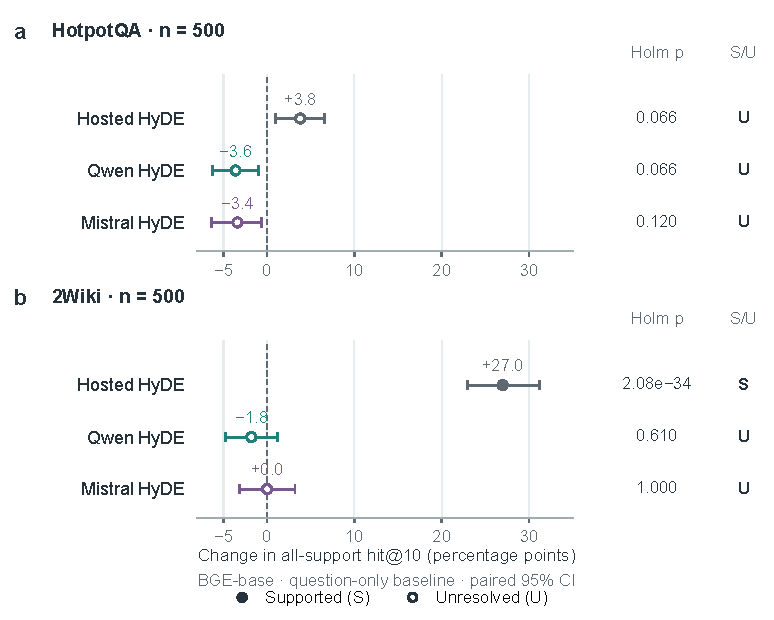
\includegraphics[width=\textwidth]{Fig2_GeneratorContrasts.pdf}
\caption{Generator-conditioned retrieval contrasts. Standard HyDE minus question-only all-support hit@10 with BGE-base on the processed local (a) HotpotQA and (b) 2Wiki corpora, each with 500 questions. Points and bars show paired effects and reported 95\% bootstrap intervals in percentage points. Filled (S) and hollow (U) points preserve supported and unresolved decisions from the original Holm families, not a newly pooled six-row family. All HotpotQA decisions remain unresolved despite intervals excluding zero. Hosted/local differences include implementation and output budgets.}
\label{fig:generator_contrasts}
\end{figure}


The BGE-prefix intervention changes all-support by at most 1.2 percentage points. All four intervals include zero and adjusted McNemar values are at least 0.7183, supplying no supported explanation for the open-generator result (Online Resource 1, Section~\SuppRef{sec:supp_plan_b_sensitivity}).

The evidence hierarchy is therefore three-level: executable pinned-local evidence, an artifact-level hosted positive control, and overlap/answer-absent/scrubbing diagnostics that delimit but do not certify independence from benchmark knowledge.

\noindent\textbf{Answer to RQ2.} The two pinned open generators do not reproduce the hosted positive point-estimate direction. Their mutual contrast and the corrected Mistral-versus-Dense test remain unresolved; this does not rank hosted and open families generally.

\subsection{RQ3: Full-Wiki Retrieval and Reader Robustness}
\label{sec:rq3_fullwiki_reader}

The initial HotpotQA full-wiki comparison tests OneR/BM25, one-generation HyDE-BM25, and official-code IRCoT on one index. Their all-support hit@10 values are 0.298, 0.348, and 0.354 (Table~\ref{tab:ircot_fullwiki_main}). IRCoT improves over OneR by $+0.056$ ($[0.012,0.100]$; Holm-adjusted McNemar $p=0.0369$), but differs from HyDE by only $+0.006$ ($[-0.042,0.056]$; $p=0.8732$). IRCoT averages 2.104 retrieval/generation rounds.

\begin{table*}[t]
\centering
\caption{HotpotQA full-wiki retrieval, serialized evidence, reader outcomes, and structural cost on the same 500 questions. ``Full para.'' requires every complete annotated supporting paragraph to remain after per-document truncation; dashes mark a paragraph-retention audit not repeated for the later learned-reranker row.}
\label{tab:ircot_fullwiki_main}
\scriptsize
\setlength{\tabcolsep}{4pt}
\textbf{A. Retrieval and evidence interface}\par\vspace{2pt}
\begin{tabularx}{\textwidth}{>{\raggedright\arraybackslash}X rrrrr}
\toprule
Condition & All title@10 & Full para. 450 & Full para. 900 & Ret. calls & Query gen. \\
\midrule
OneR/BM25 & 0.298 & 0.112 & 0.288 & 1.000 & 0.000 \\
HyDE-BM25 & 0.348 & 0.102 & 0.332 & 1.000 & 1.000 \\
Official IRCoT + Qwen & 0.354 & 0.140 & 0.340 & 2.104 & 2.104 \\
BM25 + BGE-base rescore & 0.460 & 0.176 & 0.434 & 1.000 & 0.000 \\
BM25 + BGE reranker v2-m3 & 0.468 & -- & -- & 1.000 & 0.000 \\
\bottomrule
\end{tabularx}

\vspace{5pt}
\textbf{B. Frozen evidence under two readers}\par\vspace{2pt}
\begin{tabular}{lrrrr}
\toprule
Condition & Qwen EM & Qwen F1 & Mistral EM & Mistral F1 \\
\midrule
OneR/BM25 & 0.220 & 0.2815 & 0.148 & 0.2674 \\
HyDE-BM25 & 0.236 & 0.3017 & 0.170 & 0.3032 \\
Official IRCoT + Qwen & 0.262 & 0.3366 & 0.160 & 0.2920 \\
BM25 + BGE-base rescore & 0.270 & 0.3469 & 0.186 & 0.3372 \\
BM25 + BGE reranker v2-m3 & 0.264 & 0.3480 & 0.208 & 0.3476 \\
\bottomrule
\end{tabular}
\par\smallskip
\parbox{0.97\textwidth}{\footnotesize Exact title and exact title--paragraph coverage coincide in the four interface-audited rows. Full-paragraph retention is conservative because the aligned artifact lacks official supporting-sentence IDs. Each method has one final reader call. BGE-base is retained as a separately labeled bi-encoder sensitivity comparator; the learned cross-encoder was evaluated with both readers.}
\end{table*}


The registered learned comparator, \texttt{BAAI/bge-reranker-v2-m3}, cross-encodes each question--paragraph pair in the frozen BM25 top-100 pools. It obtains any-hit/all-support/recall of 0.948/0.468/0.708. Its all-support improvements over OneR, HyDE, and IRCoT are $+0.170$ ($[0.136,0.206]$), $+0.120$ ($[0.076,0.162]$), and $+0.114$ ($[0.064,0.164]$); all three paired binary tests remain significant after Holm correction. The earlier BGE-base bi-encoder rescore reaches 0.460 and Qwen EM/F1 of 0.270/0.3469. Its retrieval score is only $0.008$ below the cross-encoder ($[-0.002,0.020]$), so the cross-encoder's advantage over the cheaper bi-encoder is unresolved.

The cross-encoder improves EM over BM25 by $+0.044$ for Qwen ($[0.014,0.074]$; $p_{\mathrm{Holm}}=0.0214$) and $+0.060$ for Mistral ($[0.032,0.090]$; $p_{\mathrm{Holm}}=0.0003$). Table~\ref{tab:ircot_fullwiki_main} preserves absolute EM/F1. Against IRCoT, Qwen EM is unresolved ($+0.002$; $[-0.040,0.042]$), while Mistral gains $+0.048$ ($[0.014,0.082]$). The cross-reader interaction for its BM25 gain is unresolved ($-0.016$; $[-0.046,0.016]$), so supported gains for both readers do not establish invariant effect sizes. Full F1 effects and paired statistics appear in Online Resource 1, Section~\SuppRef{sec:supp_plan_b_sensitivity}.
The earlier reader-by-method interaction remains unresolved: for IRCoT versus HyDE, the Qwen-minus-Mistral interaction is $+0.036$ EM ($[-0.004,0.074]$; exact sign-flip $p_{\mathrm{Holm}}=0.2562$). Reader-specific point estimates therefore do not establish a statistically reliable reader-by-method interaction.

The independent 2Wiki tier gives a narrower corpus-scale result (Table~\ref{tab:2wiki_corpus_scale}). On the 428,395-paragraph split-union corpus, BM25, Qwen-HyDE, IRCoT, and the cross-encoder obtain all-support hit@10 of 0.346, 0.356, 0.342, and 0.400. The cross-encoder has a supported retrieval gain over BM25 of $+0.054$ ($[0.032,0.078]$; $p_{\mathrm{Holm}}=2.23\times10^{-5}$). The verified S1 matrix supports this retrieval contrast on the two tested corpus configurations. HyDE ($+0.010$; $[-0.014,0.032]$) and IRCoT ($-0.004$; $[-0.052,0.042]$) likewise remain unresolved. The cross-encoder's answer gains over BM25 remain unresolved for Qwen (EM $+0.014$; $[-0.016,0.044]$) and Mistral (EM $+0.008$; $[-0.012,0.028]$). The observed retrieval increase is therefore configuration-specific and does not support a cross-dataset answer-superiority claim.

\begin{table*}[t]
\centering
\caption{Transport check on the independent split-union corpus frozen from the official 2Wiki release. The corpus-scale tier is not a second complete Wikipedia snapshot.}
\label{tab:2wiki_corpus_scale}
\scriptsize
\setlength{\tabcolsep}{3pt}
\resizebox{\textwidth}{!}{%
\begin{tabular}{lrrrrrr}
\toprule
Method & All-support@10 & Recall@10 & Qwen EM & Qwen F1 & Mistral EM & Mistral F1 \\
\midrule
BM25 OneR & 0.346 & 0.671 & 0.212 & 0.224 & 0.052 & 0.164 \\
Qwen-HyDE & 0.356 & 0.665 & 0.186 & 0.209 & 0.056 & 0.162 \\
IRCoT + Qwen & 0.342 & 0.654 & 0.218 & 0.246 & 0.072 & 0.185 \\
BGE reranker v2-m3 & 0.400 & 0.705 & 0.226 & 0.244 & 0.060 & 0.172 \\
\bottomrule
\end{tabular}
}
\end{table*}


Scorer/adapter sensitivity and official-code stopping deviations, including the retained hard-cap row, are documented in Online Resource 1, Sections~\SuppRef{sec:supp_metric_normalization} and~\SuppRef{sec:ircot_fullwiki}.

\noindent\textbf{Answer to RQ3.} Cross-encoder retrieval gains are supported on both corpus-scale tiers, but answer gains are supported for both readers only on HotpotQA. Both 2Wiki answer decisions remain unresolved.

\subsection{RQ4: IRCoT Round-Budget Sensitivity}
\label{sec:rq4_round_budget}

The round-prefix analysis asks how the frozen IRCoT trajectory changes after one round, after two rounds, and at its natural or capped exit. It is a sensitivity analysis, not a strict equal-budget comparison: later prefixes contain more retrieved documents and more generation calls, and questions may stop at different rounds. From round 1 to round 2, all-support hit rises from 0.158 to 0.344 ($+0.186$; $[0.152,0.220]$), EM from 0.166 to 0.254 ($+0.088$; $[0.062,0.116]$), and F1 by $+0.0981$ ($[0.0710,0.1264]$). Holm-adjusted exact tests remain significant for retrieval ($p<10^{-27}$) and EM ($p<10^{-9}$); the complete round table appears in Online Resource 1.

The increment from round 2 to the full trajectory is much smaller: all-support increases by $+0.010$ ($[0.002,0.020]$), EM by $+0.008$ ($[0.002,0.016]$), and F1 by $+0.0077$ ($[0.0017,0.0154]$). The corresponding adjusted exact tests are not significant ($p=0.0625$ for all-support and $p=0.125$ for EM). Most measured benefit therefore arrives by the second round under this configuration, whereas later adaptive continuation has a small average point gain. One retained hard-cap example and its post-hoc sentence-boundary sensitivity are documented in Online Resource 1, Section~\SuppRef{sec:ircot_fullwiki} and do not alter aggregates.

\noindent\textbf{Answer to RQ4.} Most observed gain arrives by round two under unequal accumulated cost; this does not establish an optimal stopping rule.

\subsection{External News-Corpus Validation: MultiHop-RAG}
\label{sec:mhrag_external}

MultiHop-RAG~\cite{tang2024multihoprag} supplies a news-document benchmark outside the Wikipedia-oriented tiers. The complete frozen release has 2,556 questions: retrieval and answer EM/F1 use 2,255 non-null questions; 301 null queries define separate canonical abstention. Support is matched by parent-document evidence IDs, rather than Wikipedia titles. Five available retrieval methods, two pinned readers and both 450/900-character evidence settings yield 20 sealed cells with 51,120 answers.

This is an available-condition analysis, not a complete six-condition transfer test. IRCoT is technically unavailable because the frozen local adapter assumes the HotpotQA corpus/index and lacks registered external parser, prompt, stopping and smoke anchors. This limits the implementation, not the IRCoT algorithm. Four observed contrasts versus BM25 use Holm correction with a fifth slot reserved conservatively at 1.0; no observed IRCoT $p$-value is imputed. The full registered family and transport decision are not complete.

% Generated by scripts/build_jiis_chatfix_tables.py; available evidence only.
\begin{table*}[!htbp]
\centering\footnotesize
\caption{MultiHop-RAG retrieval on 2,255 non-null queries (top-10).}
\label{tab:mhrag_retrieval}
\begin{threeparttable}
\setlength{\tabcolsep}{3pt}
\begin{tabular}{lrrrrlr}
\toprule
Method & Any & All & Recall & $\Delta$All & 95\% CI & $p_{\rm Holm}$ \\
\midrule
BM25 & 0.982 & 0.583 & 0.807 & -- & -- & -- \\
Dense BGE & 0.979 & 0.503 & 0.767 & -0.079 & [-0.098, -0.060] & $<0.001$ \\
Qwen-HyDE & 0.970 & 0.448 & 0.731 & -0.134 & [-0.155, -0.114] & $<0.001$ \\
Mistral-HyDE & 0.968 & 0.434 & 0.718 & -0.149 & [-0.169, -0.128] & $<0.001$ \\
Cross-encoder & 0.996 & 0.729 & 0.890 & +0.146 & [+0.127, +0.165] & $<0.001$ \\
\bottomrule
\end{tabular}
\begin{tablenotes}\scriptsize\item Parent-document evidence IDs define support; 301 null queries are excluded from retrieval denominators. Cross-encoder reranks a frozen BM25 top-100 pool. All-support and EM are primary endpoints. Four observed contrasts versus BM25 use Holm correction with a fifth slot conservatively reserved at 1.0 for unavailable IRCoT; this is not an observed IRCoT $p$-value. The full registered family is incomplete. Intervals are 95\% question-level bootstrap intervals (10,000 resamples); intervals alone do not determine significance.
\end{tablenotes}
\end{threeparttable}
\end{table*}


Complete-support retrieval is \MHRBMAll{} for BM25, \MHRDenseAll{} for Dense, \MHRQAll{} for Qwen-HyDE and \MHRMAll{} for Mistral-HyDE. All three adjusted contrasts with BM25 are negative. The cross-encoder reaches \MHRCEAll{}, with a positive adjusted gain of \MHRCEGain{} (Table~\ref{tab:mhrag_retrieval}). Standard open-generator expansion therefore supplies no observed gain over the lexical baseline here, while reranking the frozen BM25 top-100 pool does.

New post-hoc comparisons also match each expansion directly to the same Dense baseline on all 2,255 non-null IDs. All-support deltas are $-0.0550$ for Qwen-HyDE and $-0.0692$ for Mistral-HyDE, with Holm-adjusted $p=2.29\times10^{-11}$ and $3.24\times10^{-17}$. All eight reader/length EM comparisons favor Dense after adjustment. These additional families leave the historical BM25 family unchanged (Online Resource 1, Section~\SuppRef{sec:supp_priority_diagnostics}).

Retrieval improvement only partly carries through to answers. Cross-encoder EM gains over BM25 are positive after adjustment with both readers at 450 characters and Qwen at 900 characters; Mistral/900 remains unresolved. Both HyDE variants have negative adjusted EM contrasts with Qwen at both lengths; their Mistral contrasts are unresolved. Dense improves Mistral/900 EM, with the other EM contrasts unresolved. The exploratory EM interaction is significant only for Mistral-HyDE versus BM25 at 450 characters. Non-significant interactions do not establish reader invariance. Both lengths, secondary F1, raw/adapted scores and null abstention are retained in supplementary Section~\SuppRef{sec:supp_mhrag_external} in Online Resource 1.

Figure~\ref{fig:retrieval_answer_contrasts} summarizes the cross-encoder contrasts with BM25 across the three corpus-scale evaluations. Retrieval gains are supported in each, whereas the answer decisions depend on corpus, reader and, for news, character budget. The distinct support definitions and endpoints preclude a pooled gain or retrieval-to-answer conversion rate.

\begin{figure}[tbp]
\centering
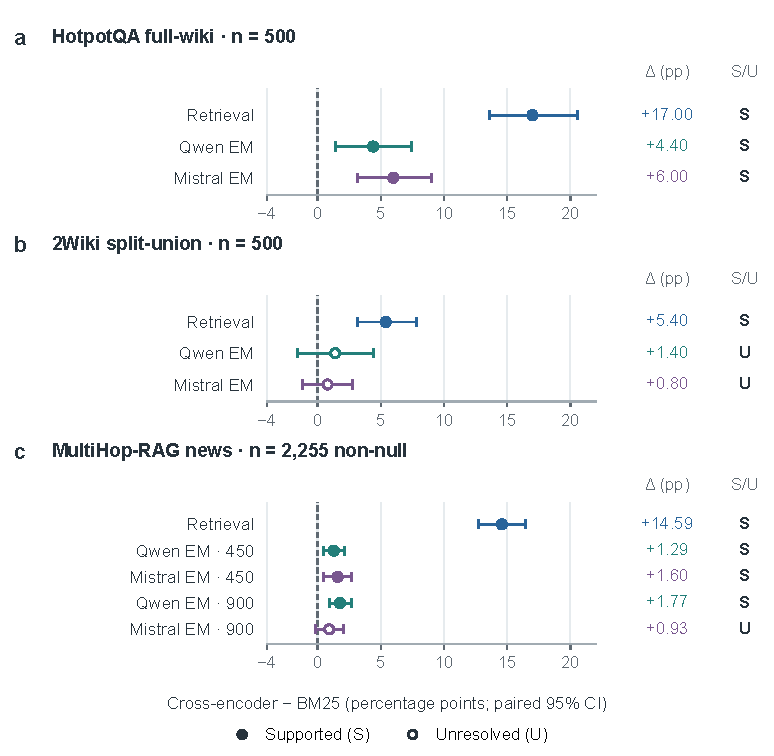
\includegraphics[width=\textwidth]{Fig3_RetrievalAnswer.pdf}
\caption{Retrieval and answer gains across evaluated configurations. Cross-encoder minus BM25 paired effects and reported 95\% bootstrap intervals on (a) HotpotQA full-wiki, (b) 2Wiki split-union and (c) MultiHop-RAG news. Retrieval is all-support hit@10; answer quality is exact match (EM). News labels 450/900 denote characters per document; retrieval is drawn once. Filled (S) and hollow (U) points preserve original Holm decisions. Wiki support uses titles; news support uses parent-document evidence IDs and excludes 301 null questions. Effects are not pooled across endpoints or corpora and do not estimate causal mediation.}
\label{fig:retrieval_answer_contrasts}
\end{figure}


Null queries expose a separate reader limitation. Mistral/900 canonical abstention is 0.0299 for both BM25 and the cross-encoder, compared with Qwen at 0.6611/0.6213. However, lexical refusal expressions occur in 170/301 and 153/301 Mistral outputs, respectively. This gap and frequent output-cap termination indicate a format-sensitive endpoint, rather than a human-confirmed hallucination rate. The registered adapter and canonical-null scores remain unchanged.

On the frozen 500-question prompt subset, query2doc-style improves all-support retrieval over standard for both generators after adjustment; evidence-only does not. Same-subset Dense and BM25 scores are 0.502 and 0.590, versus 0.516/0.512 for Qwen/Mistral Query2doc-style. The new 36-contrast post-hoc family leaves both Query2doc-versus-Dense comparisons unresolved and both contrasts with BM25 negative. Seed dispersion on the disjoint 300-question subset remains descriptive; alternative-prompt answer gains are unmeasured. Missing end-to-end costs prevent efficiency claims, and withdrawn independent human validation leaves evidence sufficiency unmeasured.


\subsection{Evidence-Interface Audit}
\label{sec:evidence_interface_audit}

Figure~\ref{fig:evidence_retention} distinguishes retrieved supporting titles, retained annotated sentences and retained full paragraphs under two character budgets. The original frozen-label audit has title and annotated-paragraph completeness coinciding before serialization. At 450 characters, complete paragraphs remain verbatim for 0.112/0.102/0.140/0.176 of questions for OneR, HyDE, IRCoT and BGE-base; at 900 characters the rates are 0.288/0.332/0.340/0.434 (Table~\ref{tab:ircot_fullwiki_main}).

The retrospective official-sentence audit uses the same 500 IDs and retains all annotated sentences for 0.254/0.284/0.298/0.388 of questions at 450 characters (Online Resource 1, Table~\SuppRef{tab:supporting_sentence_audit}). One official supporting-title set differs from the frozen labels; Figure~\ref{fig:evidence_retention} consistently uses official labels and preserves the primary results.

A final-input audit includes the learned cross-encoder and both reader templates on these 500 IDs. All 5,000 actual 450-character inputs remain below 2,000 tokens, with reconstructed prompts matching stored hashes. Cross-encoder annotated-sentence completeness falls from 0.470 at retrieval to 0.390 after character serialization, with no further token-stage loss. The other methods retain 0.254/0.284/0.298/0.388 under both readers. Historical effective-token hashes were not recorded, so inputs are reconstructed. The earlier 500-question 900-character audit is counterfactual; actual matched-budget answers are reported below. Retention does not establish factual sufficiency (Online Resource 1, Section~\SuppRef{sec:supp_priority_diagnostics}).

\begin{figure}[tbp]
\centering
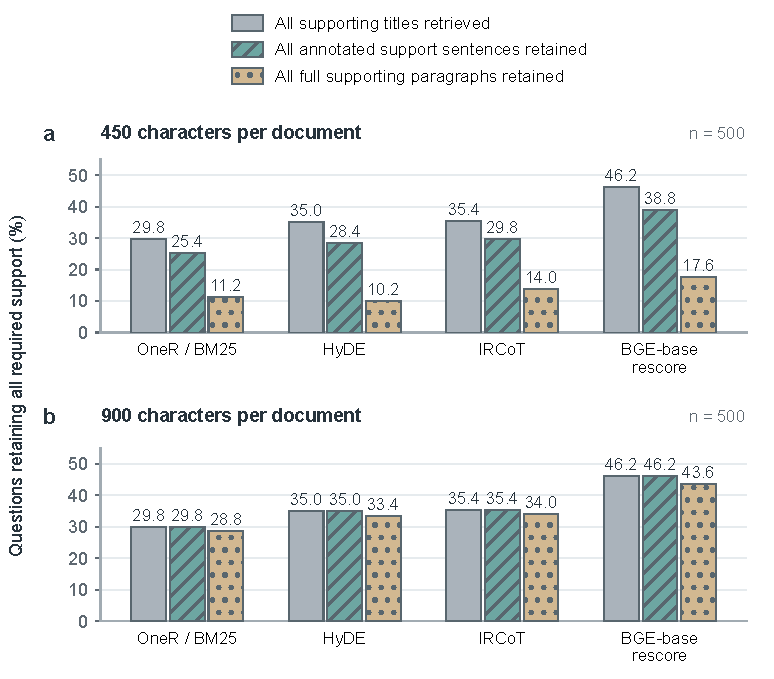
\includegraphics[width=\textwidth]{Fig4_EvidenceRetention.pdf}
\caption{Annotated evidence retention under (a) 450 and (b) 900 characters per document. Bars show complete-support question rates on 500 frozen HotpotQA IDs using the official retrospective sentence-audit labels consistently: all supporting titles retrieved, all annotated sentences retained and all full supporting paragraphs retained. One official title set differs from the primary labels; original scores remain unchanged (Online Resource 1, Section~\SuppRef{sec:supp_sentence_audit}). BGE-base rescore is a bi-encoder, distinct from Figure~\ref{fig:retrieval_answer_contrasts}. Coverage precedes global token clipping and does not establish human sufficiency. Bars are descriptive.}
\label{fig:evidence_retention}
\end{figure}


A matched intervention then generates 400 fresh answers on the first 100 original questions with fixed cross-encoder evidence, comparing 450 and 900 characters under the same suffix-preserving input policy. Complete support retention rises from 46\% to 55\%, with no token-stage clipping. Qwen EM remains 0.29 ($\Delta=0$; 95\% CI $[-0.05,0.05]$); Mistral changes from 0.22 to 0.21 ($\Delta=-0.01$; $[-0.06,0.03]$). Neither EM nor F1 establishes a gain: both separately specified two-test families have adjusted $p=1$ for each reader. Increased annotated-support delivery therefore does not guarantee improved answer scores in this diagnostic. Actual token amounts differ; it is neither an equal-cost comparison nor independent validation (Online Resource 1, Section~\SuppRef{sec:supp_followup_serializer}).

\subsection{Reader Controls and New-sample Validation}
\label{sec:new_reader_controls_results}
On the fixed 100-question subset, Qwen EM is 0.09 without supplied evidence and 0.57 with complete gold-selected support. Historical same-ID BM25/cross-encoder EM is 0.18/0.29. Mistral gives 0.05/0.35 without evidence/with gold support, versus 0.15/0.22 for BM25/cross-encoder. Local and official EM coincide for these comparisons, although F1 conventions differ.

Gold support improves Qwen EM over the cross-encoder by $+0.28$ [$0.18,0.38$], with adjusted $p=1.36\times10^{-5}$. Mistral's $+0.13$ [$0.02,0.24$] remains unresolved after adjustment ($p=0.0702$). The ten-contrast EM family includes both readers and all five fixed comparisons per reader. Gold-selected support improves both readers over question-only, yet neither reaches perfect EM. These controls expose remaining benchmark-answer errors without assigning them uniquely to reasoning, formatting or retrieval. Full outputs and termination diagnostics appear in Online Resource 1, Table~\SuppRef{tab:priority_reader_controls}.

A separate 64-question dev check excludes all 500 previously observed project IDs. The frozen retrieval-mean and audit-informed rules both select the cross-encoder before new outcomes. Shared selected-policy EM is 0.2813 for Qwen and 0.2188 for Mistral. Complete annotated support falls from 33/64 retrieved to 24/64 after character serialization, with no additional token loss. The identical choices yield structural zero performance increment, with no inferential test or general method-selection advantage (Online Resource 1, Section~\SuppRef{sec:supp_independent_validation_new}).

\subsection{Implementation and Validation Synthesis}
\label{sec:implementation_validation_synthesis}

The named local contrasts (Table~\ref{tab:boundary_stability_matrix}) support reranker retrieval over BM25 in the tested HotpotQA and 2Wiki configurations; 2Wiki answer gains remain unresolved. A deterministic reporting-rule analysis of 32 unique observed primary effects gives 19 favorable and 13 adverse point estimates, versus 12 supported, seven rejected and 13 unresolved effects using their original Holm families (Online Resource 1, Table~\SuppRef{tab:claim_stress}). Seven favorable point estimates remain unresolved after correction. This is descriptive re-expression, without new tests or a measure of framework accuracy. Five unavailable external IRCoT slots are excluded from observed counts; they still constrain transport. Framework positioning from primary papers is reported in Online Resource 1, Table~\SuppRef{tab:framework_comparison}.

\subsection{Complete Comparison on Random New Questions}
\label{sec:followup_holdout_results}
The new 300-question full-wiki matrix (Online Resource 1, Section~\SuppRef{sec:supp_followup_holdout}) runs all three methods under both readers. Complete-support retrieval is 0.350/0.440/0.537 for BM25/HyDE/CE; all three paired improvements are supported. CE-minus-BM25 EM is $+0.090$ for Qwen (CI $[0.050,0.130]$, $p_{\mathrm{Holm}}=0.000152$) and $+0.070$ for Mistral ($[0.030,0.110]$, $p=0.003764$). HyDE-minus-BM25 EM is supported for Qwen ($+0.060$, $p=0.011740$) and unresolved for Mistral ($+0.0167$, $p=0.499560$). CE-minus-HyDE EM is unresolved for Qwen and supported for Mistral; both secondary F1 contrasts are supported. These local decisions do not test a reader interaction. Complete annotated support reaches actual input in only 86/103/121 questions, with no further token-stage loss. New means remain separate from historical results and use the official single answer; same-source random new IDs do not establish contamination-free or cross-dataset validation.

\subsection{Failure Analysis and Artifact Availability}
\label{sec:failure_analysis}

Online Resource 1, Table~\SuppRef{tab:evidence_completeness_buckets_supp} separates answers by support completeness, while Table~\SuppRef{tab:single_annotator_error_taxonomy} describes retrieval, reasoning and surface-form errors. The latter is a single-annotator diagnostic, not a validated annotation benchmark; full case records and qualitative examples are reported in Online Resource 1, Sections S16--S17.

The allowlisted capsules reconstruct summary tables, eight historical open-generator retrieval contrasts and all 31 new serializer/holdout contrasts. Missing inputs still limit news reanalysis, raw-prediction rescoring and model reruns; full boundaries appear in Online Resource 1, Section~\SuppRef{sec:supp_code_artifact_availability}.

\FloatBarrier
\section{Discussion and Limitations}
\label{sec:discussion_limitations}

The experiments separate three questions: whether expansion retrieves complete support, whether that support reaches the reader, and whether answers improve. Their different outcomes prevent a single aggregate score from establishing transport. Unresolved decisions do not establish equivalence or invariance. The audit organizes these observations using established paired inference; production reliability and a general system-selection benefit remain untested.

\subsection{Generator, Evidence and Reader Dependence}
\label{sec:generator_reader_dependence}

Hypothetical queries sample a generator's knowledge and instruction-following behavior. The same-BGE comparisons show that generator provenance matters: hosted expansions improve aggregate retrieval, while the pinned Qwen and Mistral point estimates do not. This accords with concerns about knowledge leakage~\cite{yoon2025knowledgeleakage} from benchmark content in hypothetical documents. Under BGE, the hosted exact-answer stratum has a positive effect, the supporting-entity stratum is unresolved, and the no-identifiable-content stratum is negative with an interval reaching zero. Positive MiniLM answer-absent and scrubbed aggregates therefore do not establish a content-independent mechanism. Answer-string absence cannot exclude unrecognized paraphrase, classification error, parametric memory or provider-side contamination. The alias replay additionally limits hosted evidence to the preserved artifact.

The BGE query-prefix sensitivity changes each all-support estimate by at most 1.2 percentage points, with all intervals including zero and no adjusted decision below 0.05. This particular encoder-interface change does not supply a supported explanation for the open-generator result.

At the reader interface, the HotpotQA final-input audit locates annotated-support loss at character serialization, with no additional token loss in the actual 450-character inputs. In news documents, parent identity and exact fact-span retention are distinct measurements. Cross-encoder parent completeness is 0.7286 before global token budgeting, but complete exact fact-span retention is only 0.0004 at 450 characters. At 900 characters, parent completeness falls to 0.6958 for Qwen and 0.6661 for Mistral after token budgeting. The strict lexical span diagnostic cannot exclude paraphrased or distributed evidence, yet parent recovery alone cannot certify that every gold fact reaches the reader.

The new matched 100-question character-budget intervention recovers complete support in nine additional questions without establishing answer gains. It directly checks a budget change while holding retrieval and reader fixed, but does not isolate semantic sufficiency from input length or demonstrate equivalence. Retention and answers therefore remain separate endpoints.

Cross-encoder EM gains over BM25 on HotpotQA are $+0.044$ for Qwen and $+0.060$ for Mistral, but their interaction is unresolved. Both 2Wiki answer gains are unresolved. These Wikipedia-oriented results do not establish a statistically reliable reader-by-method interaction or a common effect size. In MultiHop-RAG, adjusted cross-encoder EM gains are supported for both readers at 450 characters and only Qwen at 900. Only the Mistral-HyDE/450 EM interaction is significant in the separately labeled exploratory family. Neither isolated significance nor unresolved interactions establish general reader dependence or invariance.

The random 300-question matrix separately supports CE answer gains over BM25 with both readers. HyDE improves complete-support retrieval, but its Mistral answer gain remains unresolved. These new effects strengthen a tested local comparison rather than a general ranking, and their different adjusted decisions do not establish a reader interaction. The sample is disjoint from observed study outputs but uses the same development source; small effects remain weakly powered and training contamination is not tested.

\subsection{Cost-Aware System Choice}
\label{sec:system_design_implications}

The findings support three checks before choosing components. First, compare expansion with question-only retrieval using the same dense encoder and corpus. Its advantage over BM25 alone cannot establish that generation improves the matched representation. The negative news comparisons make this distinction consequential in the tested configurations. Second, inspect the evidence in actual reader tokens, since complete-support retrieval can coexist with losses during serialization. Third, measure same-question answer effects directly; supported retrieval gains and unresolved answer gains coexist in the 2Wiki tier. These checks identify unsupported inferences without establishing a generally superior selection policy.

The learned reranker needs no query-generation call but scores 100 question--paragraph pairs per question. Its recorded HotpotQA reranking stage took 972.5 seconds for 500 questions on an RTX 4060 Laptop GPU. Calls alone thus understate computation. Its retrieval advantage over the BGE-base bi-encoder rescore is unresolved, as is its Qwen answer difference from IRCoT. IRCoT remains a configuration-specific option when complete-support recovery warrants additional adaptive calls. The round-prefix result motivates testing a two-round cap; it does not validate an optimal stopping rule because later prefixes accumulate documents and calls.

MultiHop-RAG cost records describe successful operations and runtime cohorts. Missing generator-token counts, historical memory/failed-attempt measurements and end-to-end timing, together with reconstructed historical Qwen/450 input lengths, prevent dollar-cost, deployment-latency or causal speedup claims. Research assistants and enterprise search are motivating contexts, not evaluated deployments.

\subsection{Threats to Validity}
\label{sec:threats_to_validity}

\textbf{Data and models.} Controlled evidence comprises two 500-example English benchmarks and processed candidate pools. The shared 100k check remains benchmark-derived. HotpotQA uses one complete Wikipedia snapshot; the 428,395-paragraph 2Wiki split union is not a second complete Wikipedia snapshot. News-corpus validation does not complete IRCoT or a cross-corpus factorial. MiniLM/BGE and two locally quantized 7B instruction models do not establish results for larger models, other quantization, languages or retriever families. Hosted provenance lacks an independently verified immutable provider snapshot; hosted/local contrasts also differ in generation implementation and output caps. They cannot isolate generator architecture, scale or knowledge as a causal factor.

\textbf{Measurement and scope amendment.} Title completeness, exact paragraph retrieval, complete-paragraph retention, annotated-sentence retention and human evidence sufficiency are distinct. Official sentence arrays were acquired retrospectively from a pinned HotpotQA-hosted conversion. One question differs in official and frozen supporting titles; both views are retained without changing primary scores. EM/F1 and the narrow deterministic answer adapter can penalize valid alternatives. The older single-annotator taxonomy is illustrative. The planned 120-item independent human audit was withdrawn after automated results were available because qualified annotators could not be recruited; no labels were collected and the packet and blank forms remain archived. Human evidence sufficiency and inter-annotator reliability are unmeasured, and automated scores or model judgments cannot replace them. The original full protocol was not completed.

\textbf{Inference and implementation.} Holm adjustment is family-specific, and percentile intervals need not agree with exact-test decisions near zero; both are reported. The 32-effect stress test re-expresses existing outcomes under reporting rules, not framework accuracy or a false-positive rate. Query2doc-style and official-code/open-generator IRCoT are adaptations, not historical reproductions. Cross-encoding is conditional on frozen BM25 top-100 pools and cannot recover missed evidence outside them. BGE-base rescoring remains a bi-encoder comparator. The news reader correction preserves the answer/chat suffix under unchanged budgets, excludes malformed historical outputs and permits only verified effective-token-identical reuse.

\textbf{Release.} Versioned numerical capsules with an explicit file allowlist reconstructs summary tables and recomputes eight historical retrieval contrasts and all 31 new contrasts from sanitized metrics. Current news reader families require excluded per-question inputs for full reanalysis. Prediction rescoring and model reruns need separately acquired data, predictions, indexes and pinned weights. Historical hosted raw answers are unavailable. These checks establish bounded artifact auditability. The numerical capsules accompany the article as Online Resources 2 and 3; no archival DOI has been assigned.

\section{Conclusion}
\label{sec:conclusion}

The reported reliability boundaries are empirical limits of supported gains within the tested English configurations. They distinguish expansion gains from evidence delivery and answer gains; unresolved gains do not establish absence of an effect. The hosted HotpotQA gain does not establish a content-independent effect or transfer to either pinned open generator. On news documents, standard HyDE underperforms matched Dense retrieval and all eight reader/length EM conditions. Better prompting improves the standard condition without establishing superiority over Dense.

The learned cross-encoder has supported retrieval gains over BM25 in the Wikipedia-oriented tiers and news documents. A random 300-question comparison supports its answer gains over BM25 with both readers, while other answer decisions differ across configurations. The final-input audit confirms character-stage support loss in the actual HotpotQA reader configuration, without additional token-stage loss. A matched 100-question budget change recovers additional support without establishing answer gains. These observations identify distinct measurement boundaries; they do not establish a causal explanation or human evidence sufficiency.

The findings motivate matched question-only baselines, effective-input checks, and direct answer comparisons when evaluating expansion or reranking. Named contrasts and family-specific paired decisions make those checks inspectable within the tested English configurations. Gold-selected controls improve both readers over question-only but do not establish a causal bottleneck or strict answer upper bound. The 2Wiki split-union corpus, unavailable external IRCoT, incomplete end-to-end costs and withdrawn independent human audit constrain generalization. New-sample validation does not establish a selection benefit when competing frozen rules select the same method. The study therefore provides neither a universal account of when expansion works nor a validated predictive model or method-selection rule; transport to untested configurations requires further evaluation.


\section*{Statements and Declarations}
\begingroup
\footnotesize

\noindent\textbf{Funding.} This research received no project funding.\par
\noindent\textbf{Competing interests.} The authors declare no competing interests.\par
\noindent\textbf{Author contributions.} Xingyun Chen: conceptualization, methodology, software, investigation, formal analysis, writing---original draft, and writing---review and editing. Shiyong Xiong: supervision.\par
\noindent\textbf{Ethics approval.} Not applicable. This study used public benchmark materials and model experiments; no human participants were recruited and no personal data were collected. Authors' case checks were limited to public materials.\par
\noindent\textbf{Consent to participate.} Not applicable; no human participants were recruited.\par
\noindent\textbf{Consent for publication.} Not applicable; this article reports no identifiable participant information.\par
\noindent\textbf{Data availability.} HotpotQA, 2WikiMultihopQA and MultiHop-RAG are available from their original providers under their terms. Sanitized numeric inputs for eight historical retrieval contrasts and 31 new paired contrasts accompany the article in Online Resources 2 and 3. These exclude benchmark text, raw predictions and indexes. Full news-reader reanalysis, prediction rescoring and model reruns require additional per-question inputs, upstream data and model weights; the supplied vectors do not replace these inputs.\par
\noindent\textbf{Code availability.} Online Resources 2 and 3 contain versioned reconstruction/reanalysis code (0.1.0-local-20261004 and 0.2.0-local-20261004), manifests and instructions. Project-authored software is covered by the included MIT license; third-party data and models retain their own terms. These packages reproduce the specified tables and numeric contrasts, not full model runs. The numerical packages are also publicly available at \url{https://github.com/creator-perterson/hyde-multihop-rag-reproducibility}, commit \texttt{a68aaaa}. Full model-running code and inputs are not included in these packages. No archival DOI has been assigned.
\endgroup

\setlength{\bibsep}{0pt}
\renewcommand{\bibfont}{\fontsize{8}{9}\selectfont}
\begin{multicols}{2}
\bibliography{references_jiis}
\end{multicols}

\end{document}
